\chapter{Evaluation} \label{cha:evaluation}

In \Cref{cha:labels} and \Cref{cha:retinas}, we examined the quality of generation of each part of the system in isolation.
Having having done this, we return to the overarching goal of this project: to observe the effect of \emph{fully-synthetic} data (i.e. generated retinas from generated semantic labels) on downstream tasks.
Hence, in the evaluation phase we aim to answer the following questions:
\begin{itemize}
    \item How closely does synthetic data resemble the real data?
    \item What effect does synthetic data have on lesion segmentation performance?
    \item What effect does synthetic data have on grading performance?
\end{itemize}

\section{Preliminary Results} \label{sec:prelim}

An early version of this project was submitted as a short paper\footnote{What qualifies as a ``short paper'' can be found at \url{https://2021.midl.io/call-for-papers.html}.} to MIDL 2021.
While using similar techniques, this work focused on generation of only the optic disc and hard exudate lesions, with the retina being added afterwards using a circle mask, in the same way as discussed above.
These preliminary results were promising, and showed that inflating real data with synthetic data was successful in improving the performance of semantic segmentation for lesions.

Despite this, the results of the paper were limited in that restricting the problem domain in this way made the task far easier, and naturally allowed for more stable training.
This was not only reflected in the generated image quality, in that the GAN was able to generate more plausible semantic labels, but also in the level of conditioning.
Here, we extend those models to generate 9 classes (from 3), and provide a more complete evaluation.

\section{Visual Quality}

\begin{figure}[h]
    \centering
    \begin{subfigure}{0.31\textwidth}
        \centering
        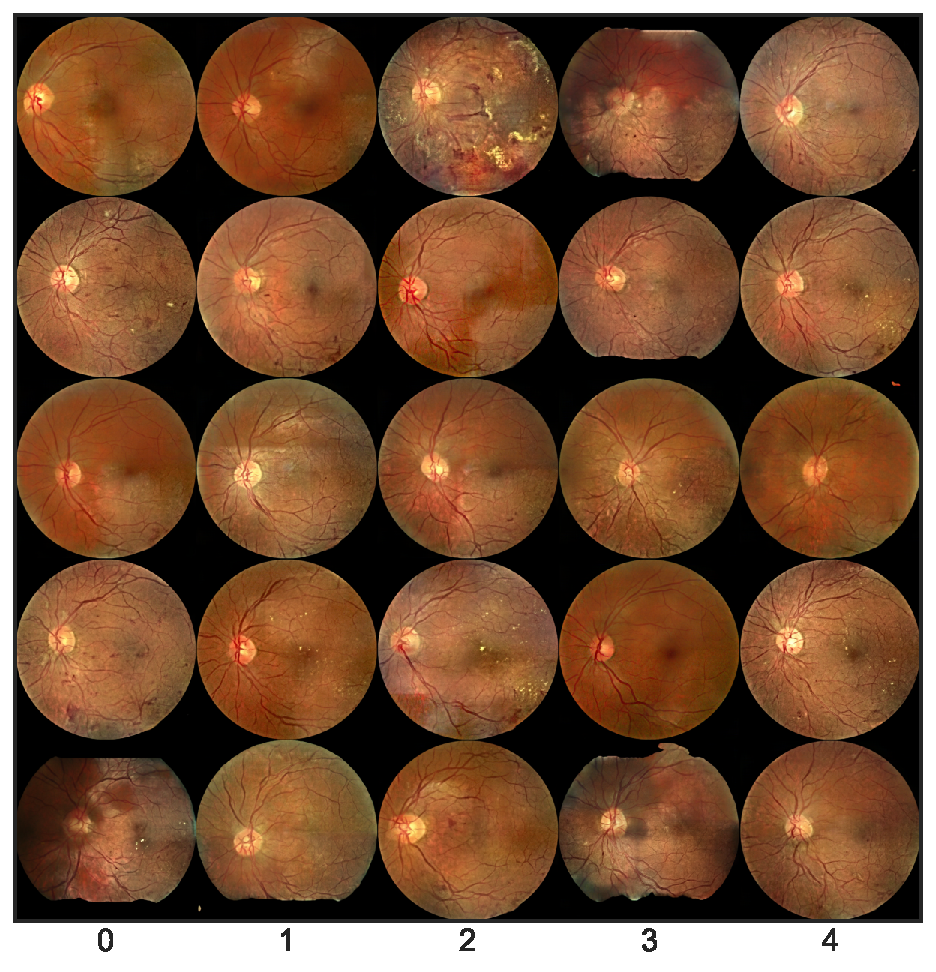
\includegraphics[width=\linewidth]{evaluation/figs/acgan_retina_sample.pdf}
        \caption{ACGAN}
        \label{fig:generated_retinas_acgan}
    \end{subfigure}
    \begin{subfigure}{0.31\textwidth}
        \centering
        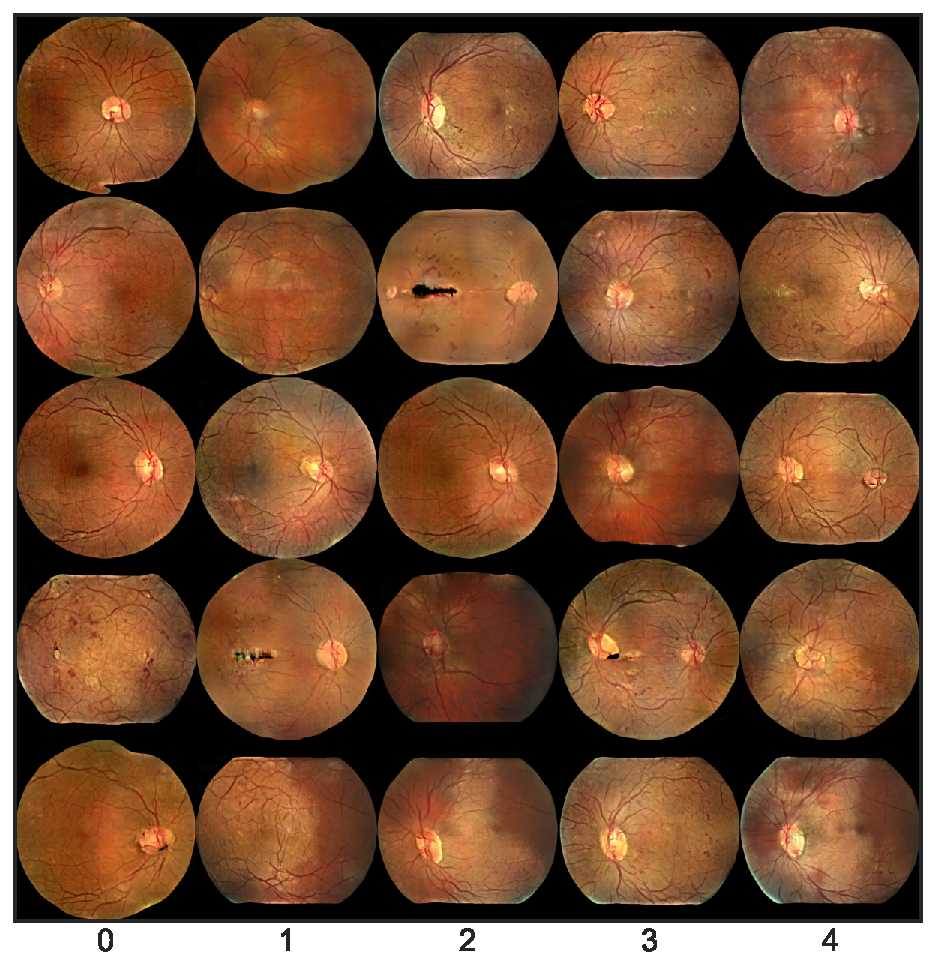
\includegraphics[width=\linewidth]{evaluation/figs/progan_retina_sample.pdf}
        \caption{ProGAN}
        \label{fig:generated_retinas_progan}
    \end{subfigure}
    \begin{subfigure}{0.31\textwidth}
        \centering
        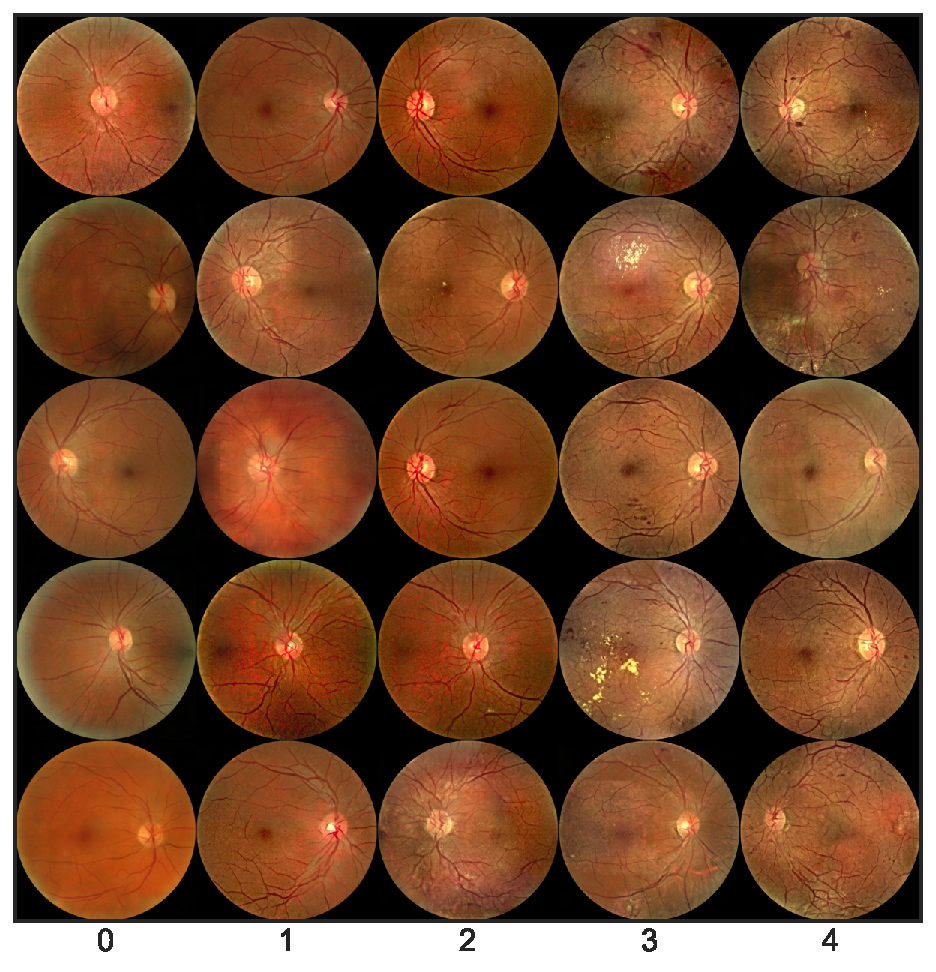
\includegraphics[width=\linewidth]{evaluation/figs/copypaste_retina_sample.pdf}
        \caption{Copy-Paste}
        \label{fig:generated_retinas_copypaste}
    \end{subfigure}
    \caption{Fully-synthetic retinal fundus images.}
    \label{fig:generated_retinas}
\end{figure}

We begin by qualitatively and quantitatively evaluating the overall visual quality of the fully-synthetic images.
A sample of images, created using each semantic label generation method, are shown in \Cref{fig:generated_retinas}.
For all experiments in this evaluation, we use the ACGAN and ProGAN generated samples without any fundus masking, unless otherwise specified.
The semantic labels are translated into retinal fundus images using the same trained SPADE network for each method with instance maps.

Curiously, images that have few lesions resemble photographs taken from the e-ophtha dataset most closely.
This is likely because most photographs of healthy retinas come from the e-ophtha dataset, and this bias is reflected in the output of the SPADE network, highlighting the need for greater diversity in the source data.

To quantify differences in diversity and quality, we begin by generating 3000 samples of fully-synthetic images in equal proportions across the five DR grades using each of the methods.
We then compute the FID score between these and the retinal fundus photographs from the training set, with results shown in \Cref{tab:spade_generated}. 
We are particularly interested in how these compare in relation to real images; to this end, the FID between the real training set and real validation/test sets are also given.

Surprisingly, the images who had their retina boundaries masked post-generation performed worse than their unmodified counterparts -- despite them performing better in the semantic label evaluation.
The reason for this is not entirely clear, but we can put forward a couple of theories.
One possible reason is that the FID score is simply not designed for these types of images, and thus gives spurious results that would be inconsistent with human perception.
In particular, purely geometric shapes such as the circle that forms the retinal fundus boundary are rare in the real world, and could be thought of as ``unnatural''.
Moreover, in the masked images these boundaries are only ever perfect circles, whereas in the source dataset, samples whose top and bottom sections have been cropped are common, which could cause distance between the data distributions.

\begin{table}[h]
    \centering
    \begin{tabular}{lrr}
        \toprule
        Configuration & \multicolumn{2}{r}{FID$\downarrow$} \\
        \midrule
        Test & 23.281 & \\
        Validation & 23.491 & \\
        \midrule
        ACGAN & \textbf{43.042} & $\pm$ 0.196 \\
        + mask & 50.642 & $\pm$ 0.229 \\
        \midrule
        ProGAN & 48.882 & $\pm$ 0.305 \\
        + mask & 54.353 & $\pm$ 0.092 \\
        \midrule
        Copy-Paste & 45.394 & $\pm$ 0.072 \\
        \bottomrule
    \end{tabular}
    \caption{FID scores between real images from the training set and the output of SPADE on the generated semantic labels. We report the mean of three runs and the standard error of the mean. Raw data can be found in \Cref{cha:raw_data}. Best results for each metric in bold (excluding the baseline).}
    \label{tab:spade_generated}
\end{table}

\section{Classification Performance}

The intuition for the first part of our classification performance evaluation is that images that closely resemble their source class should be able to be labelled correctly by a classifier trained on real data. 
To quantify this, we use the standard precision, recall, and $F_1$ score metrics.

Next, we investigate two different approaches to using synthetic data \emph{together} with real data to augment model performance.
In the first, we train models on a mix of real and generated data.
As part of this, we investigate the effects that varying the amount of synthetic data used, in terms of the proportion of the training data which is synthetic, has on the final model performance.
Each experiment will use the entire set of real training data, and only the amount of synthetic data will be tuned.
From the generated data, we sample the appropriate number of images according to the experiment, and concatenate this with the real training data.
\Cref{tab:synthetic_proportions_classification} shows how much synthetic data is used in each classification experiment -- note how for these experiments, we use the smaller grading set instead of the EyePACS dataset, since EyePACS is extremely large and therefore slow to train on.
We also considered an alternative approach where we simply take a small subset of the EyePACS dataset, but we found that the class imbalance and high amount of noise in the parent dataset (which would usually be offset by the large volume of data) caused extremely poor performance on the test set.

\begin{table}[h]
    \centering
    \begin{tabular}{rrrr}
       \toprule
       \# Real & \% Synthetic & \# Synthetic & \# Total \\
       \midrule
       \multirow{3}*{1606} & 25 & 535 & 2141 \\ 
       & 50 & 1606 & 3212 \\ 
       & 75 & 4818 & 6424 \\ 
       \bottomrule
    \end{tabular}
    \caption{Data amounts for classification experiments.}
    \label{tab:synthetic_proportions_classification}
\end{table}

The second approach is related to transfer learning.
In this particular version of the technique, we will pre-train a network on only synthetic data (7000 images) for 100 epochs, and then subsequently fine-tune on only real data for a further 100 epochs.
We are interested in determining what the effect is on both how fast the model improves on real data, and if the final performance is changed.
To contrast and compare the merits of both approaches, we collect performance metrics on the test set for each configuration, and compare these against a model trained on real data only.

Our classification network is a ResNet-50 trained to classify $512\times 512$ illumination-corrected retinal fundus images as one of the five DR grades.
Across all experiments, the network is trained for 100 epochs (where training loss plateaued) with learning rate $\alpha = 0.001$, and batch size 16, on a mix of single Nvidia Titan X Pascal and Nvidia GeForce GTX 1080 GPUs.
Each configuration is trained from scratch, with the exception of the fine-tuning stage of the transfer learning experiment.
We refer to models trained on real data only as ``baseline'' models.

\subsection{Results}

\begin{table}[h]
    \centering
    \begin{tabular}{lrrrrr}
    \toprule
        Configuration & Accuracy$\uparrow$ & Precision$\uparrow$ & Recall$\uparrow$ & $F_1$$\uparrow$ & $\kappa$$\uparrow$ \\
    \midrule 
    Validation & 0.517 & 0.455 & 0.437 & 0.435 & 0.569 \\
    Test & 0.509 & 0.442 & 0.441 &0.430 & 0.539 \\
    \midrule
        ACGAN & 0.202 & 0.196 & 0.201 & 0.164 & $-0.006$ \\
    \midrule
        ProGAN & 0.199 & 0.216 & 0.200 & 0.159 & $-0.002$ \\
    \midrule
        Copy-Paste & \textbf{0.313} & \textbf{0.366} & \textbf{0.313} & \textbf{0.247} & \textbf{0.315} \\
    \bottomrule
    \end{tabular}
    \caption{Performance of a classification model trained with only real data on real and synthetic datasets. Mean of three runs, raw data can be found in \Cref{cha:raw_data}. Best results for each metric in bold (excluding the baseline).}
    \label{tab:classification_performance}
\end{table}

The results of the real classifier on synthetic data are shown in \Cref{tab:classification_performance}.
These figures are somewhat surprising, with all types of synthetic data unable to be well-classified by the ResNet.
We expected that the copy-paste generated data would perform best out of the synthetic datasets, since its semantic labels were able to be accurately classified (\Cref{tab:acgan_results}), and this expectation is confirmed by the data.
However, even if copy-paste generated data performed the best out of the synthetic datasets, it performs poorly relative to the real validation and test sets.
Since the semantic labels of copy-pasted data were able to be classified well, it could be that performance here is being bottlenecked by the image-to-image translation portion of the generation process.

\begin{table}[h]
    \centering
    \begin{tabular}{lrr@{}lr@{}lr@{}lr@{}lr@{}l}
    \toprule
        Configuration & \% Synthetic & Accuracy$\uparrow$ & & Precision$\uparrow$ & & Recall$\uparrow$ & & $F_1$$\uparrow$ & & $\kappa$$\uparrow$ & \\
    \midrule
    Real & 0 & 0.509 & & 0.442 & & 0.441 & & 0.430 & & 0.539 & \\
    \midrule
    \multirow{3}*{ACGAN} & 25 & 0.400 & & 0.440 & & 0.366 & & 0.324 & & 0.292 & \\
                         & 50 & 0.428 & & 0.467 & * & 0.414 & & 0.366 & & 0.328 & \\
                         & 75 & 0.386 & & 0.338 & & 0.302 & & 0.253 & & 0.281 & \\
    \midrule
    \multirow{3}*{ProGAN} & 25 & 0.519 & * & 0.491 & * & 0.506 & * & 0.477 & * & 0.631 & * \\
                          & 50 & 0.410 &   & 0.470 & * & 0.436 & & 0.360 & & 0.525 & \\
                          & 75 & 0.570 & * & 0.487 & * & 0.409 & & 0.395 & & 0.489 & \\
    \midrule
    \multirow{3}*{Copy-Paste} & 25 & 0.502 & & 0.462 & * & 0.479 & * & 0.448 & * & 0.607 & * \\
                              & 50 & 0.561 & * & \textbf{0.533} & * & \textbf{0.566} & * & \textbf{0.522} & * & \textbf{0.721} & * \\
                             & 75 & \textbf{0.599} & * & 0.522 & * & 0.536 & * & 0.511 & * & 0.703 & * \\
    \bottomrule
    \end{tabular}
    \caption{Performance of a classification model trained with mixed data on the test set. Mean of three runs, raw data can be found in \Cref{cha:raw_data}. Best results for each metric in bold (excluding the baseline), and improvements on the baseline are marked with *.}
    \label{tab:classification_mixed_performance}
\end{table}

Next, we conduct experiments by training the classifier on a mix of real and synthetic data, with results shown in \Cref{tab:classification_mixed_performance}.
This set of results are less surprising, with the ACGAN unanimously causing classification performance to drop.
A small amount of synthetic data generated from the ProGAN appears to be beneficial, slightly boosting the classification metrics at 25\% synthetic data, above which performance begins to fall.
Meanwhile, training on a mix of real and copy-pasted data is able to significantly boost classification performance.
What is most noteworthy here is how copy-pasted data can increase performance by a large margin when mixed with real data, yet is not able to be accurately classified by a model trained on only real data.
Both the ACGAN and copy-paste configurations observe a peak at 50\% synthetic data, with 25\% and 75\% performing worse.
This suggests that increasing the amount of synthetic data will improve model performance to a critical point, after which the model with begin to overfit to unrealistic features in the synthetic data.
The models used in these experiments were trained over between one and eleven hours each, depending on the size of the training set.

\begin{table}[h]
    \centering
    \begin{tabular}{llr@{}lr@{}lr@{}lr@{}lr@{}l}
    \toprule
        \multicolumn{2}{c}{Configuration} & Accuracy$\uparrow$ & & Precision$\uparrow$ & & Recall$\uparrow$ & & $F_1$$\uparrow$ & & $\kappa$$\uparrow$ & \\
    \midrule
    Real & & 0.509 & & 0.442 & & 0.441 & & 0.430 & & 0.539 & \\
    \midrule
    \multirow{2}*{Copy-Paste} & Pre-Trained & \textbf{0.605} & * & \textbf{0.559} & * &  \textbf{0.534} & * & \textbf{0.529} & * & \textbf{0.694} &* \\
               & Fine-Tuned & 0.566 & * & 0.555 & * & 0.525 & * & 0.512 & * & 0.660 & * \\
    \bottomrule
    \end{tabular}
    \caption{Performance of a classification model on the test set before and after fine-tuning. Mean of three runs, raw data can be found in \Cref{cha:raw_data}. Best results for each metric in bold (excluding the baseline), and improvements on the baseline are marked with *.}
    \label{tab:classification_transfer}
\end{table}

Finally, we look at how transfer learning affects the ability of the model to classify images correctly.
We only use copy-pasted data for pre-training since it appears to be most effective for this task, and the results of these experiments are shown in \Cref{tab:classification_transfer}.
Here, ``pre-trained'' refers to the network once it has finished training on only synthetic data, and ``fine-tuned'' refers to the same network once it has finished further training on real data.
The results are unexpected, with the synthetic-only model performing \emph{better} on the test set than the fine-tuned network.
A possible explanation for this is that the real dataset is small, and has noisy DR severity labels.
Images generated by copy-pasting are the result of sampling semantic labels from multiple different images of the same grade, causing the classes to be more robust, and therefore less noisy.
Both the pre-trained and fine-tuned networks perform better than training on only real data, which implies that pre-training increases the ability of the model to extract useful features.
The pre-trained model is able to outperform the baseline and fine-tuned models, but its $\kappa$ falls short of the copy-paste mixed-data training approach, despite having a slightly more favourable $F_1$ score.
This is a consequence of the quadratic weighting used to calculate $\kappa$, but we maintain use of $\kappa$ as the determining factor of ``overall'' performance.

It is also interesting to analyse the resulting loss curves of transfer learning, and to compare these against the losses of a network trained on only real data, as shown in \Cref{fig:classification_transfer_loss}.
The loss in the pre-training stage decreases slowly, which makes sense since the greater volume of synthetic data (which could be thought of as a type of data augmentation) has a regularising effect on training.
Once the network enters the fine-tuning stage, the model is able to leverage its past experience, and begins training at a much lower loss than the one trained from scratch.
Despite this ``head-start'', the baseline model's loss decreases quickly, and by the end of training is approximately the same magnitude as the fine-tuned network.
The effect of transfer learning on the validation loss is more subtle, and there is no clear difference between the losses of the baseline and fine-tuned models.

\begin{figure}[h]
    \centering
    \begin{subfigure}{0.45\textwidth}
        \centering
        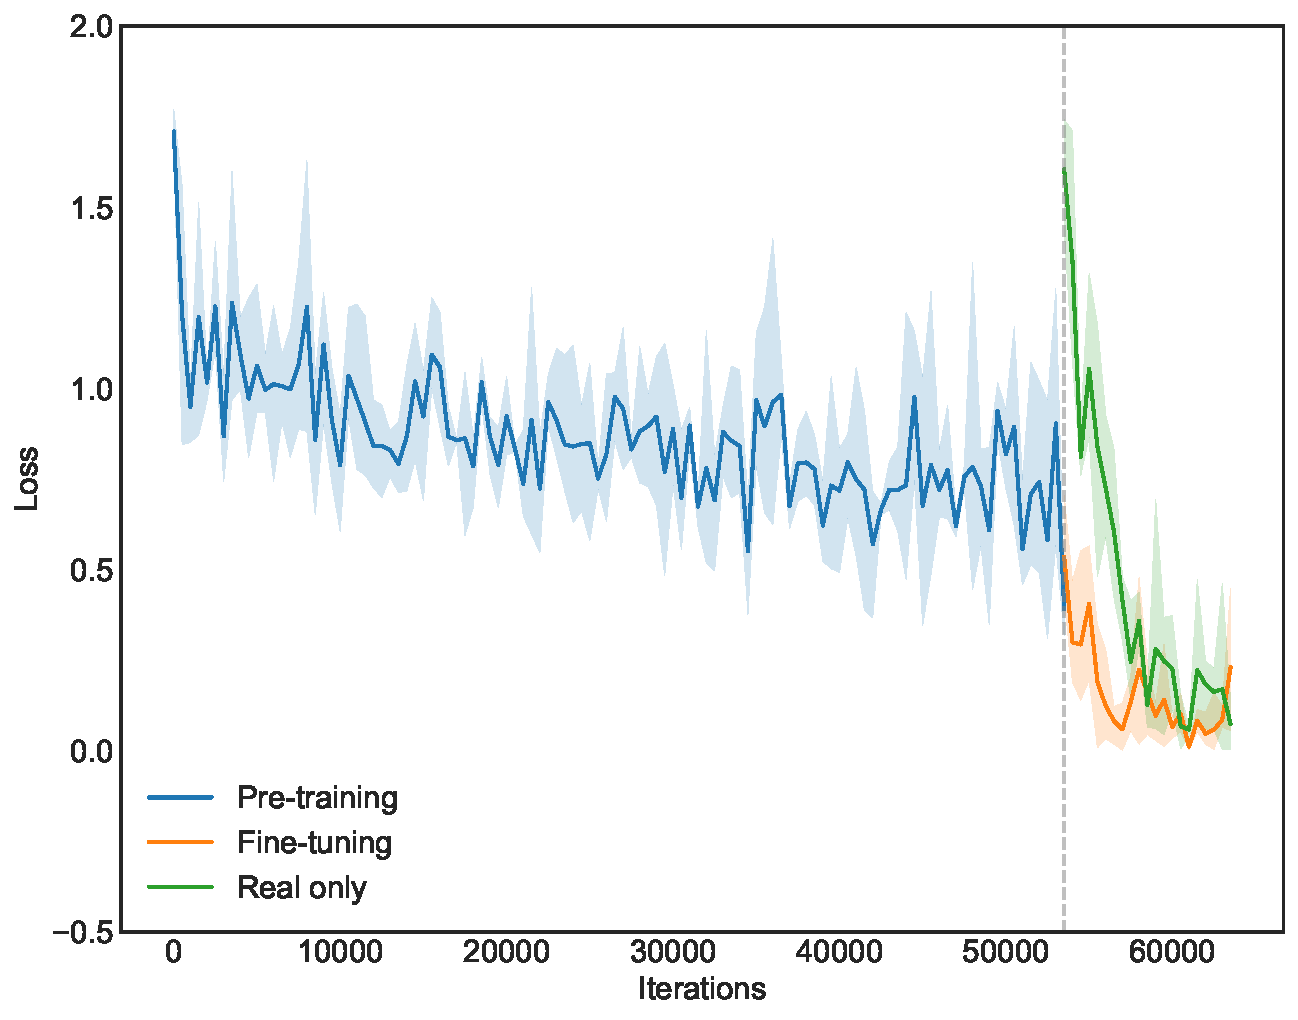
\includegraphics[width=\linewidth]{evaluation/figs/transfer_training_loss.pdf}
        \caption{Training loss.}
        \label{fig:classification_transfer_loss_training}
    \end{subfigure}
    \begin{subfigure}{0.45\textwidth}
        \centering
        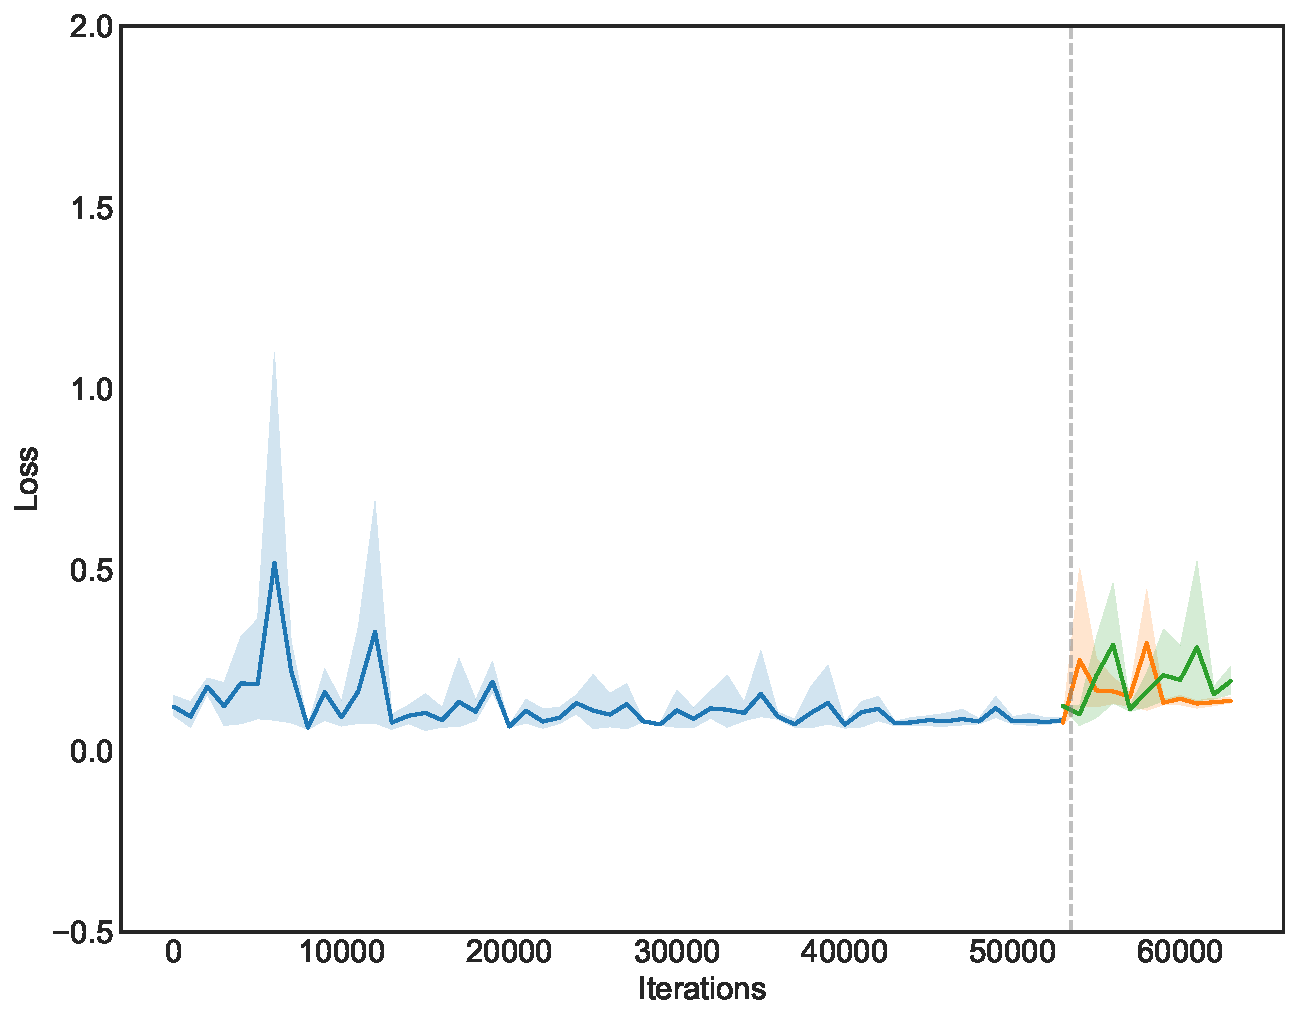
\includegraphics[width=\linewidth]{evaluation/figs/transfer_validation_loss.pdf}
        \caption{Validation loss.}
        \label{fig:classification_transfer_loss_validation}
    \end{subfigure}
    \caption{Loss curves for transfer learning. Solid lines are the means of three runs, and the shaded regions show the minimum and maximum values.}
    \label{fig:classification_transfer_loss}
\end{figure}

\section{Segmentation Performance}

\begin{table}[h]
    \centering
    \begin{tabular}{rrrr}
       \toprule
       \# Real & \% Synthetic & \# Synthetic & \# Total \\
       \midrule
       \multirow{3}*{1607} & 25 & 536 & 2143 \\ 
       & 50 & 1607 & 3214 \\ 
       & 75 & 4821 & 6428 \\ 
       \bottomrule
    \end{tabular}
    \caption{Data amounts for segmentation experiments.}
    \label{tab:synthetic_proportions_segmentation}
\end{table}

Applying a similar principle to the segmentation task: if our model produces clear and well-conditional retinal fundus images with precise segmentation maps, a model should be able to segment our synthesised images about as well as it can segment real images. 
We then go on to investigate the same two approaches to training on synthetic data as described in the previous section.
For the mixed-data approach, we use use the proportions specified in \Cref{tab:synthetic_proportions_segmentation}.

A standard U-Net is used as our segmentation model architecture.
Models were trained to segment all six lesion types (microaneurysms, haemorrhages, hard exudates, soft exudates, intraretinal microvascular abnormalities, and neovascularistion) at a resolution of $512 \times 512$.
They do not segment other structures such as the optic disc or fundus boundary.
All models were trained for 50 epochs with a learning rate of $\alpha = 0.0005$ and batch size of 4 on a mix of single Nvidia Titan X Pascal and Nvidia GeForce GTX 1080 GPUs.
We focus on the \emph{relative} performance as opposed to the absolute performance, and therefore do not spend time optimising the model hyperparameters.

\subsection{Results}

\begin{table}[h]
    \centering
    \begin{tabular}{lrrr}
    \toprule
        Configuration & Precision$\uparrow$ & Recall$\uparrow$ & $F_1$$\uparrow$ \\
    \midrule 
    Test & 0.710 & 0.400 & 0.439 \\
    Validation & 0.690 & 0.374 & 0.434 \\
    \midrule
        ACGAN & 0.662 & 0.200 & 0.278 \\
    \midrule
        ProGAN & 0.754 & 0.183 & 0.523 \\
    \midrule
        Copy-Paste & \textbf{0.808} & \textbf{0.462} & \textbf{0.527} \\
    \bottomrule
    \end{tabular}
    \caption{Performance of a segmentation model trained with only real data on real and synthetic datasets. Mean of three runs, raw data can be found in \Cref{cha:raw_data}. Best results for each metric in bold (excluding the baseline).}
    \label{tab:segmentation_performance}
\end{table}

\Cref{tab:segmentation_performance} shows the results of running the baseline segmentation model trained with real data on the synthetic datasets.
We find that the model performs best across all metrics on the copy-pasted data, followed closely by the ProGAN.
The overall performance (as determined by the $F_1$ score) for both of these models is greater than that of the test and validation sets.
This is indicative of plausible generated semantic labels and well-conditioned image-to-image translation.
Performance on the ACGAN generated data, however, is significantly poorer than for any other dataset.

\begin{table}[h]
    \centering
    \begin{tabular}{lrr@{}lr@{}lr@{}l}
        \toprule
        Configuration & \% Synthetic & Precision$\uparrow$ & & Recall$\uparrow$ & & $F_1$$\uparrow$ & \\
        \midrule
        Real & 0 & 0.710 & & 0.400 & & 0.439 & \\
        \midrule
        \multirow{3}*{ACGAN} & 25 & 0.688 & & 0.368 & & 0.421 & \\
              & 50 & 0.608 & & 0.353 & & 0.406 & \\
              & 75 & \textbf{0.723} & * & 0.412 & * & 0.473 & * \\
        \midrule
        \multirow{3}*{ProGAN} & 25 & 0.687 & & 0.400 & & 0.449 & *\\
               & 50 & 0.662 & & \textbf{0.482} & * & 0.464 & * \\
               & 75 & 0.685 & & 0.406 & * & 0.461 & * \\
        \midrule
        \multirow{3}*{Copy-Paste} & 25 & 0.716 & * & 0.297 & & 0.364 & \\
                   & 50 & 0.702 & & 0.392 & & 0.452 & * \\
                   & 75 & 0.689 & & 0.423 & * & \textbf{0.476} & *\\
        \bottomrule
    \end{tabular}
    \caption{Performance of a segmentation model trained with mixed data on the test set. Mean of three runs, raw data can be found in \Cref{cha:raw_data}. Best results for each metric in bold (excluding the baseline), and improvements on the baseline are marked with *.}
    \label{tab:segmentation_mixed_performance}
\end{table}

Turning our attention to experiments conducted with mixed training data, \Cref{tab:segmentation_mixed_performance} shows the performance of the segmentation model trained under varying amounts of synthetic data.
The results are extremely promising, showing that segmentation performance can be boosted by training on synthetic data.
We identify an interesting trend where increasing the amount of synthetic data simultaneously decreases precision while increasing recall.
The overall effect of this is that the $F_1$ score improves, at least up to 75\% synthetic data. 
We can think of precision as ``how many selected items are relevant`` and recall as ``how many relevant items are selected''; hence, decreased precision and increased recall can be interpreted as the resulting model being more ``liberal'' with its selection.
It's likely that, as with the classification experiments, this relationship reaches a point where the $F_1$ score begins to decrease, but further experiments are required to verify this. 

\begin{table}[h]
    \centering
    \begin{tabular}{llr@{}lr@{}lr@{}l}
        \toprule
        \multicolumn{2}{c}{Configuration} & Precision$\uparrow$ & & Recall$\uparrow$ & & $F_1$$\uparrow$ & \\
        \midrule
        Real & & 0.710 & & 0.400 & & 0.439 & \\
        \midrule
        \multirow{2}*{Copy-Paste} & Pre-Trained & 0.646 & & \textbf{0.453} & * & \textbf{0.510} &* \\
               & Fine-Tuned & \textbf{0.729} & * & 0.420 & * & 0.501 & * \\
        \bottomrule
    \end{tabular}
    \caption{Performance of a segmentation model on the test set before and after fine-tuning. Mean of three runs, raw data can be found in \Cref{cha:raw_data}. Best results for each metric in bold (excluding the baseline), and improvements on the baseline are marked with *.}
    \label{tab:segmentation_transfer_performance}
\end{table}

This trend continues with the transfer learning approach, where the pre-trained network exhibits a higher recall but lower precision than the baseline model, with a greater overall $F_1$ score.
Conversely, continuing training on the real data has the inverse effect of increasing precision and decreasing recall.
Again, we see parallels with the transfer learning approach applied to classification in that the $F_1$ score is better on the pre-trained model than the fine-tuned model, as if seeing real data causes performance to drop.
Both the pre-trained and fine-tuned models are able to achieve a greater $F_1$ score than any of the baseline or mixed-data training approaches, suggesting that this is the optimal strategy to maximise segmentation performance.

Looking at the loss curves in \Cref{fig:segmentation_transfer_loss}, we see a similar pattern to the classification transfer learning loss, although training loss actually increases when entering the fine-tuning stage, suggesting the model has overfit on the synthetic data.

\begin{figure}[h]
    \centering
    \begin{subfigure}{0.45\textwidth}
        \centering
        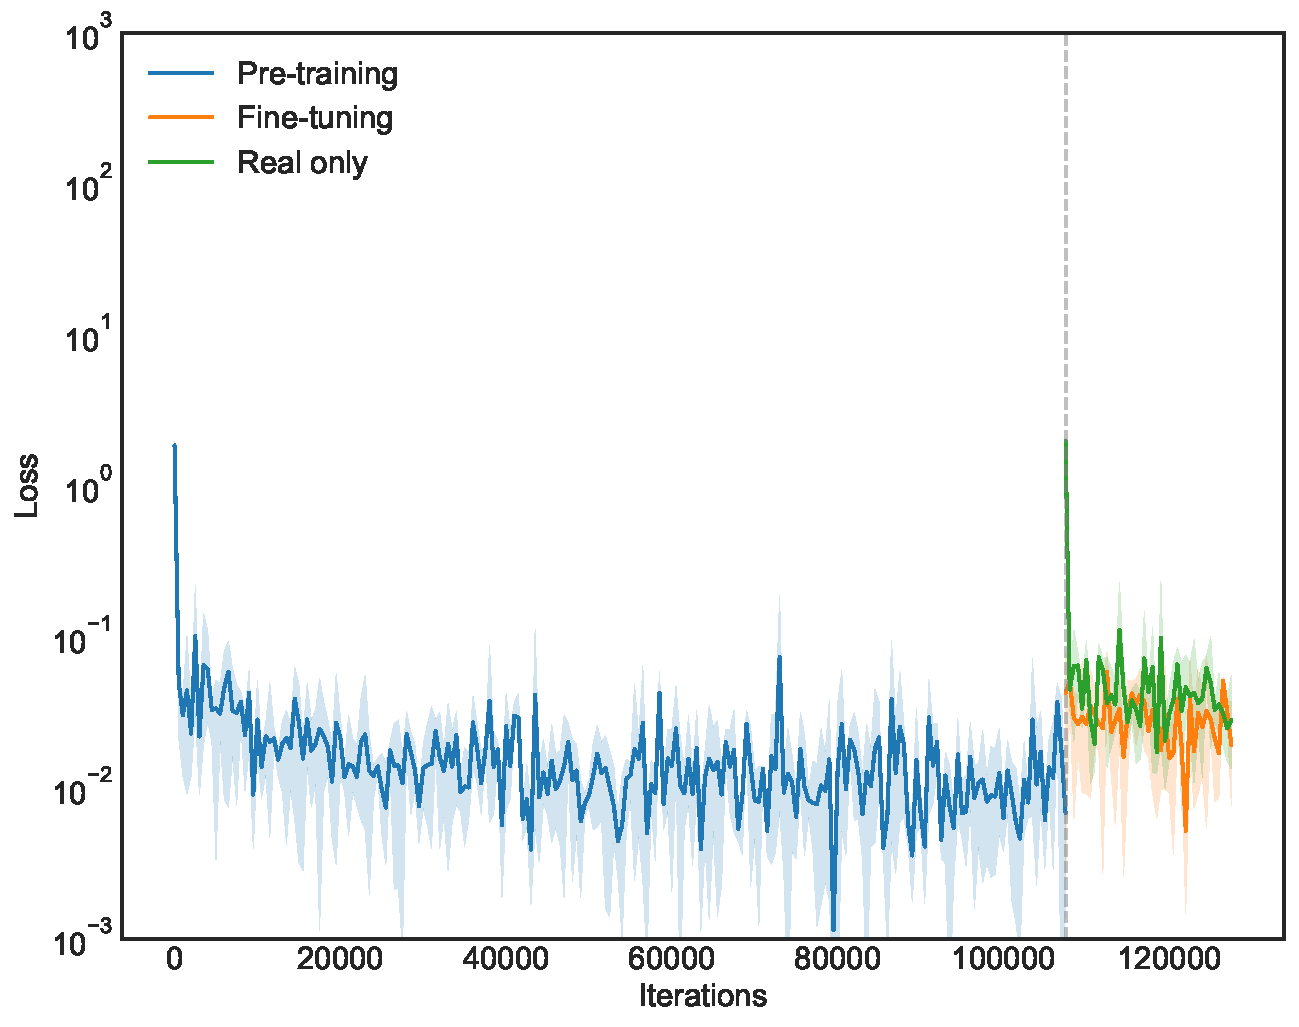
\includegraphics[width=\linewidth]{evaluation/figs/segmentation_transfer_training_loss.pdf}
        \caption{Training loss.}
        \label{fig:segmentation_transfer_loss_training}
    \end{subfigure}
    \begin{subfigure}{0.45\textwidth}
        \centering
        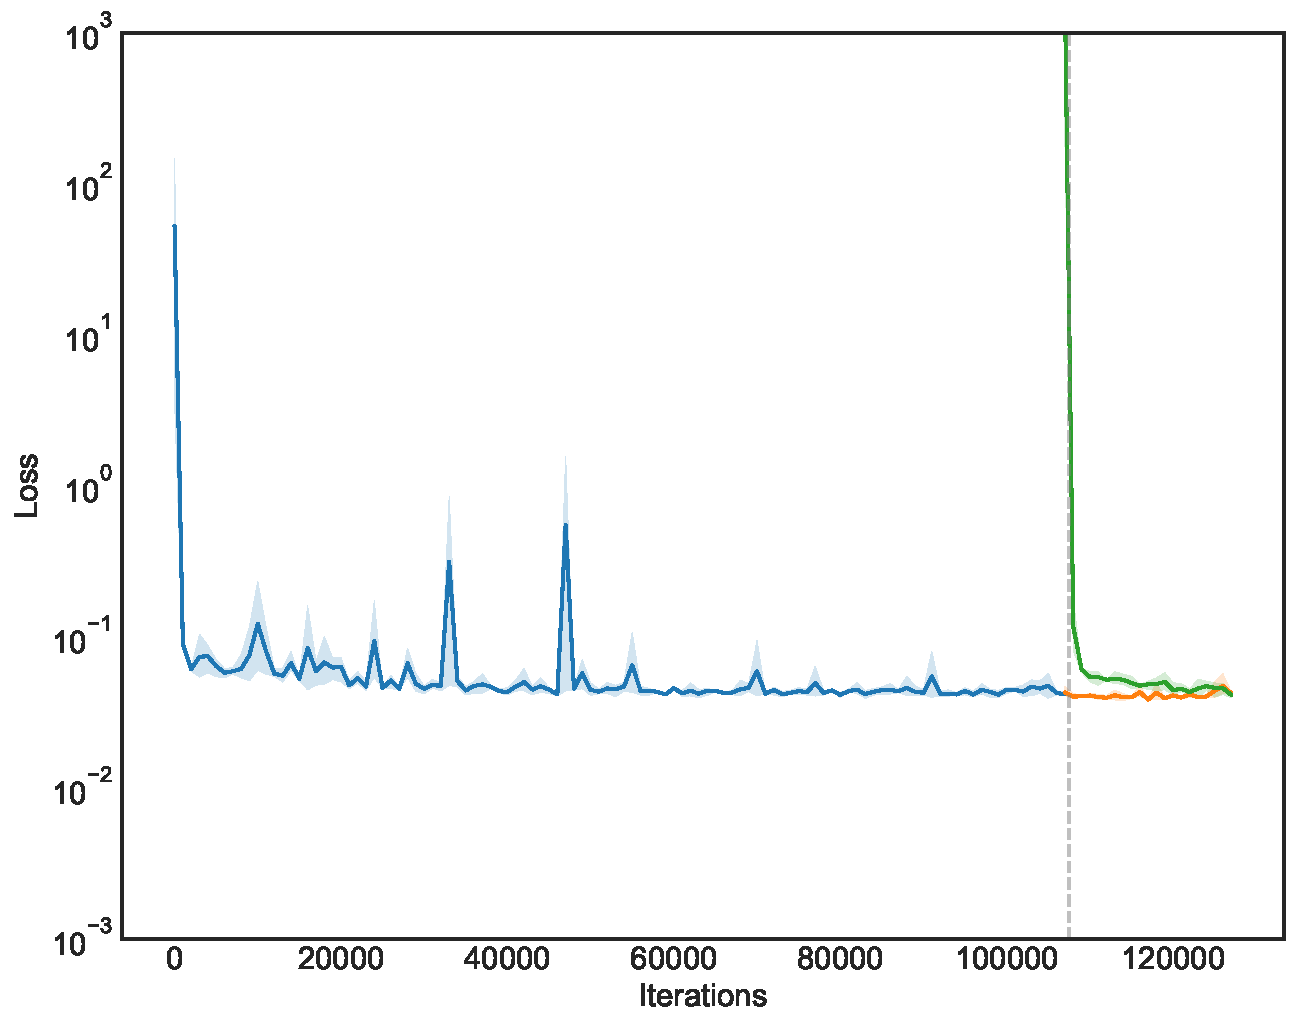
\includegraphics[width=\linewidth]{evaluation/figs/segmentation_transfer_validation_loss.pdf}
        \caption{Validation loss.}
        \label{fig:segmentation_transfer_loss_validation}
    \end{subfigure}
    \caption{Loss curves for transfer learning, plotted on a logarithmic scale. Solid lines are the means of three runs, and the shaded regions show the minimum and maximum values.}
    \label{fig:segmentation_transfer_loss}
\end{figure}